\documentclass[10pt]{article}
\usepackage[letterpaper,margin=1in]{geometry}
\usepackage[T1]{fontenc}
\usepackage{lmodern,microtype,amsmath,booktabs,graphicx,tabularx,xcolor,url}
\usepackage[hidelinks]{hyperref}
\usepackage{enumitem}
\usepackage{float}
\usepackage{tikz}
\usetikzlibrary{calc,positioning,arrows.meta,fit,backgrounds}
\definecolor{figblue}{HTML}{2a78d6}
\definecolor{figorange}{HTML}{eb6834}
\definecolor{figgreen}{HTML}{008300}
\definecolor{figred}{HTML}{c03535}
\definecolor{figink}{HTML}{31302e}
\setlist{nosep,leftmargin=*}
\setlength{\parindent}{1em}
\setlength{\parskip}{0pt}
\setlength{\textfloatsep}{5pt plus 2pt minus 2pt}
\setlength{\floatsep}{4pt plus 2pt minus 2pt}
\setlength{\abovecaptionskip}{3pt}
\setlength{\belowcaptionskip}{2pt}
\renewcommand{\topfraction}{0.95}
\renewcommand{\textfraction}{0.05}
\renewcommand{\floatpagefraction}{0.8}
\usepackage{titlesec}
\titlespacing*{\section}{0pt}{8pt plus 2pt minus 1pt}{4pt plus 1pt}
\titlespacing*{\paragraph}{0pt}{6pt plus 1pt}{4pt}
\raggedbottom
% GENERATED by src.analysis.h100_results -- do not edit.
\newif\ifHOneHundredComplete
\HOneHundredCompletefalse
\newif\ifHFullGridComplete
\HFullGridCompletefalse
\newif\ifHHasReportableCohort
\HHasReportableCohortfalse
\def\HProfileLabel{Deadline}
\def\HDoneCount{13}
\def\HStartedCount{8}
\def\HPendingCount{11}
\def\HCapturedUTC{2026-08-12T03:29:18+00:00}
\def\HClosedFractions{none}
\def\HHardware{NVIDIA H100 80GB HBM3}
\def\HCodeRevision{1a82d508fbeb9fdf6868a9637611e9018952fb43}
\def\HResultProfile{deadline}
\def\HResultMetricScope{corrected-development-selection}
\def\HResultCaptureUTC{2026-08-12T03:29:18+00:00}
\def\HResultCampaignID{judy-h100-operator-status-2026-08-12}
\def\HResultCodeSHA{1a82d508fbeb9fdf6868a9637611e9018952fb43}
\def\HResultHardware{NVIDIA H100 80GB HBM3}
\def\HResultPythonVersion{3.11.13}
\def\HResultTorchVersion{2.11.0+cu126}
\def\HResultCudaVersion{12.6}
\def\HResultPrecision{32-true}
\def\HResultDoneCount{13}
\def\HResultStartedCount{8}
\def\HResultPendingCount{11}
\def\HResultVerifiedCount{0}
\def\HResultReportableFractionCount{0}
\def\HResultReportableFractions{none}
\def\HResultEvidenceScope{contract-verified completed cohorts only}
\def\HDevFViTRandomHundred{\textemdash}
\def\HStatusViTRandomHundred{Done}
\def\HDevFViTOpticalHundred{\textemdash}
\def\HStatusViTOpticalHundred{Done}
\def\HDevFViTSarHundred{\textemdash}
\def\HStatusViTSarHundred{Done}
\def\HDevFViTImageNetHundred{\textemdash}
\def\HStatusViTImageNetHundred{Done}
\def\HDevFCNNRandomHundred{\textemdash}
\def\HStatusCNNRandomHundred{Done}
\def\HDevFCNNOpticalHundred{\textemdash}
\def\HStatusCNNOpticalHundred{Done}
\def\HDevFCNNSarHundred{\textemdash}
\def\HStatusCNNSarHundred{Done}
\def\HDevFCNNImageNetHundred{\textemdash}
\def\HStatusCNNImageNetHundred{Done}
\def\HDevFViTRandomFifty{\textemdash}
\def\HStatusViTRandomFifty{Done}
\def\HDevFViTOpticalFifty{\textemdash}
\def\HStatusViTOpticalFifty{Started}
\def\HDevFViTSarFifty{\textemdash}
\def\HStatusViTSarFifty{Started}
\def\HDevFViTImageNetFifty{\textemdash}
\def\HStatusViTImageNetFifty{Started}
\def\HDevFCNNRandomFifty{\textemdash}
\def\HStatusCNNRandomFifty{Done}
\def\HDevFCNNOpticalFifty{\textemdash}
\def\HStatusCNNOpticalFifty{Done}
\def\HDevFCNNSarFifty{\textemdash}
\def\HStatusCNNSarFifty{Done}
\def\HDevFCNNImageNetFifty{\textemdash}
\def\HStatusCNNImageNetFifty{Done}
\def\HDevFViTRandomTwentyFive{\textemdash}
\def\HStatusViTRandomTwentyFive{Started}
\def\HDevFViTOpticalTwentyFive{\textemdash}
\def\HStatusViTOpticalTwentyFive{Pending}
\def\HDevFViTSarTwentyFive{\textemdash}
\def\HStatusViTSarTwentyFive{Pending}
\def\HDevFViTImageNetTwentyFive{\textemdash}
\def\HStatusViTImageNetTwentyFive{Pending}
\def\HDevFCNNRandomTwentyFive{\textemdash}
\def\HStatusCNNRandomTwentyFive{Started}
\def\HDevFCNNOpticalTwentyFive{\textemdash}
\def\HStatusCNNOpticalTwentyFive{Started}
\def\HDevFCNNSarTwentyFive{\textemdash}
\def\HStatusCNNSarTwentyFive{Started}
\def\HDevFCNNImageNetTwentyFive{\textemdash}
\def\HStatusCNNImageNetTwentyFive{Started}
\def\HDevFViTRandomTen{\textemdash}
\def\HStatusViTRandomTen{Pending}
\def\HDevFViTOpticalTen{\textemdash}
\def\HStatusViTOpticalTen{Pending}
\def\HDevFViTSarTen{\textemdash}
\def\HStatusViTSarTen{Pending}
\def\HDevFViTImageNetTen{\textemdash}
\def\HStatusViTImageNetTen{Pending}
\def\HDevFCNNRandomTen{\textemdash}
\def\HStatusCNNRandomTen{Pending}
\def\HDevFCNNOpticalTen{\textemdash}
\def\HStatusCNNOpticalTen{Pending}
\def\HDevFCNNSarTen{\textemdash}
\def\HStatusCNNSarTen{Pending}
\def\HDevFCNNImageNetTen{\textemdash}
\def\HStatusCNNImageNetTen{Pending}

% GENERATED by src.analysis.heldout_results -- do not edit.
\newif\ifHevDevComplete
\HevDevCompletetrue
\newif\ifHevTestComplete
\HevTestCompletetrue
\newif\ifHevFinalEval
\HevFinalEvaltrue
\def\HevCodeSHAShort{06b2e61d}
\def\HevCohortSHAShort{a8996efd}
\def\HevHardware{NVIDIA H100 80GB HBM3}
\def\HevGPUHours{567.6}
\def\HevCohortCreatedUTC{2026-10-01T18:26:20+00:00}
\def\HevDeltaFTenViTOptical{+0.102}
\def\HevDeltaFTenViTSar{+0.094}
\def\HevDeltaFTenViTImageNet{+0.106}
\def\HevDeltaFTenCNNOptical{+0.038}
\def\HevDeltaFTenCNNSar{+0.077}
\def\HevDeltaFTenCNNImageNet{+0.090}
\def\HevDevFViTRandomTen{0.7917}
\def\HevThrViTRandomTen{0.808}
\def\HevEpochViTRandomTen{14}
\def\HevTestFViTRandomTen{0.6926}
\def\HevDevFViTRandomTwentyFive{0.8569}
\def\HevThrViTRandomTwentyFive{0.858}
\def\HevEpochViTRandomTwentyFive{24}
\def\HevTestFViTRandomTwentyFive{0.7729}
\def\HevDevFViTRandomFifty{0.8935}
\def\HevThrViTRandomFifty{0.852}
\def\HevEpochViTRandomFifty{34}
\def\HevTestFViTRandomFifty{0.8091}
\def\HevDevFViTRandomHundred{0.8996}
\def\HevThrViTRandomHundred{0.818}
\def\HevEpochViTRandomHundred{24}
\def\HevTestFViTRandomHundred{0.8306}
\def\HevDevFViTOpticalTen{0.8933}
\def\HevThrViTOpticalTen{0.901}
\def\HevEpochViTOpticalTen{49}
\def\HevTestFViTOpticalTen{0.8064}
\def\HevDevFViTOpticalTwentyFive{0.8854}
\def\HevThrViTOpticalTwentyFive{0.921}
\def\HevEpochViTOpticalTwentyFive{29}
\def\HevTestFViTOpticalTwentyFive{0.8371}
\def\HevDevFViTOpticalFifty{0.9201}
\def\HevThrViTOpticalFifty{0.938}
\def\HevEpochViTOpticalFifty{34}
\def\HevTestFViTOpticalFifty{0.8369}
\def\HevDevFViTOpticalHundred{0.9222}
\def\HevThrViTOpticalHundred{0.897}
\def\HevEpochViTOpticalHundred{44}
\def\HevTestFViTOpticalHundred{0.8567}
\def\HevDevFViTSarTen{0.8857}
\def\HevThrViTSarTen{0.587}
\def\HevEpochViTSarTen{4}
\def\HevTestFViTSarTen{0.8041}
\def\HevDevFViTSarTwentyFive{0.8624}
\def\HevThrViTSarTwentyFive{0.768}
\def\HevEpochViTSarTwentyFive{4}
\def\HevTestFViTSarTwentyFive{0.7715}
\def\HevDevFViTSarFifty{0.9184}
\def\HevThrViTSarFifty{0.878}
\def\HevEpochViTSarFifty{39}
\def\HevTestFViTSarFifty{0.8652}
\def\HevDevFViTSarHundred{0.9293}
\def\HevThrViTSarHundred{0.918}
\def\HevEpochViTSarHundred{39}
\def\HevTestFViTSarHundred{0.8861}
\def\HevDevFViTImageNetTen{0.8980}
\def\HevThrViTImageNetTen{0.849}
\def\HevEpochViTImageNetTen{39}
\def\HevTestFViTImageNetTen{0.8129}
\def\HevDevFViTImageNetTwentyFive{0.8765}
\def\HevThrViTImageNetTwentyFive{0.892}
\def\HevEpochViTImageNetTwentyFive{29}
\def\HevTestFViTImageNetTwentyFive{0.8476}
\def\HevDevFViTImageNetFifty{0.9234}
\def\HevThrViTImageNetFifty{0.859}
\def\HevEpochViTImageNetFifty{39}
\def\HevTestFViTImageNetFifty{0.8589}
\def\HevDevFViTImageNetHundred{0.9367}
\def\HevThrViTImageNetHundred{0.861}
\def\HevEpochViTImageNetHundred{44}
\def\HevTestFViTImageNetHundred{0.8509}
\def\HevDevFCNNRandomTen{0.7992}
\def\HevThrCNNRandomTen{0.716}
\def\HevEpochCNNRandomTen{29}
\def\HevTestFCNNRandomTen{0.6571}
\def\HevDevFCNNRandomTwentyFive{0.8167}
\def\HevThrCNNRandomTwentyFive{0.819}
\def\HevEpochCNNRandomTwentyFive{44}
\def\HevTestFCNNRandomTwentyFive{0.7065}
\def\HevDevFCNNRandomFifty{0.8716}
\def\HevThrCNNRandomFifty{0.846}
\def\HevEpochCNNRandomFifty{49}
\def\HevTestFCNNRandomFifty{0.7803}
\def\HevDevFCNNRandomHundred{0.9002}
\def\HevThrCNNRandomHundred{0.858}
\def\HevEpochCNNRandomHundred{39}
\def\HevTestFCNNRandomHundred{0.8155}
\def\HevDevFCNNOpticalTen{0.8371}
\def\HevThrCNNOpticalTen{0.825}
\def\HevEpochCNNOpticalTen{49}
\def\HevTestFCNNOpticalTen{0.7197}
\def\HevDevFCNNOpticalTwentyFive{0.8619}
\def\HevThrCNNOpticalTwentyFive{0.886}
\def\HevEpochCNNOpticalTwentyFive{34}
\def\HevTestFCNNOpticalTwentyFive{0.7505}
\def\HevDevFCNNOpticalFifty{0.8826}
\def\HevThrCNNOpticalFifty{0.864}
\def\HevEpochCNNOpticalFifty{39}
\def\HevTestFCNNOpticalFifty{0.8214}
\def\HevDevFCNNOpticalHundred{0.9045}
\def\HevThrCNNOpticalHundred{0.847}
\def\HevEpochCNNOpticalHundred{49}
\def\HevTestFCNNOpticalHundred{0.8405}
\def\HevDevFCNNSarTen{0.8762}
\def\HevThrCNNSarTen{0.776}
\def\HevEpochCNNSarTen{34}
\def\HevTestFCNNSarTen{0.8000}
\def\HevDevFCNNSarTwentyFive{0.8868}
\def\HevThrCNNSarTwentyFive{0.876}
\def\HevEpochCNNSarTwentyFive{14}
\def\HevTestFCNNSarTwentyFive{0.8030}
\def\HevDevFCNNSarFifty{0.8998}
\def\HevThrCNNSarFifty{0.900}
\def\HevEpochCNNSarFifty{29}
\def\HevTestFCNNSarFifty{0.8478}
\def\HevDevFCNNSarHundred{0.9068}
\def\HevThrCNNSarHundred{0.832}
\def\HevEpochCNNSarHundred{4}
\def\HevTestFCNNSarHundred{0.8221}
\def\HevDevFCNNImageNetTen{0.8889}
\def\HevThrCNNImageNetTen{0.861}
\def\HevEpochCNNImageNetTen{4}
\def\HevTestFCNNImageNetTen{0.7925}
\def\HevDevFCNNImageNetTwentyFive{0.8962}
\def\HevThrCNNImageNetTwentyFive{0.937}
\def\HevEpochCNNImageNetTwentyFive{9}
\def\HevTestFCNNImageNetTwentyFive{0.8458}
\def\HevDevFCNNImageNetFifty{0.9268}
\def\HevThrCNNImageNetFifty{0.892}
\def\HevEpochCNNImageNetFifty{34}
\def\HevTestFCNNImageNetFifty{0.8734}
\def\HevDevFCNNImageNetHundred{0.9347}
\def\HevThrCNNImageNetHundred{0.896}
\def\HevEpochCNNImageNetHundred{49}
\def\HevTestFCNNImageNetHundred{0.8876}
\def\HevTestMeanGap{0.078}
\def\HevTestInferencePrecision{32-true}
\def\HevThrMinViT{0.587}
\def\HevThrMaxViT{0.938}
\def\HevMedianBestEpochViT{34}
\def\HevMeanCellHoursViT{13.2}
\def\HevThrMinCNN{0.716}
\def\HevThrMaxCNN{0.937}
\def\HevMedianBestEpochCNN{34}
\def\HevMeanCellHoursCNN{22.3}
\def\HevCellsPrecOverRecall{14}
\def\HevCellsEarlyStopped{9}
\def\HevEpochsRunViTRandomTen{35}
\def\HevHoursViTRandomTen{3.1}
\def\HevEpochsRunViTRandomTwentyFive{45}
\def\HevHoursViTRandomTwentyFive{7.5}
\def\HevEpochsRunViTRandomFifty{50}
\def\HevHoursViTRandomFifty{14.9}
\def\HevEpochsRunViTRandomHundred{45}
\def\HevHoursViTRandomHundred{25.2}
\def\HevEpochsRunViTOpticalTen{50}
\def\HevHoursViTOpticalTen{4.2}
\def\HevEpochsRunViTOpticalTwentyFive{50}
\def\HevHoursViTOpticalTwentyFive{8.2}
\def\HevEpochsRunViTOpticalFifty{50}
\def\HevHoursViTOpticalFifty{14.8}
\def\HevEpochsRunViTOpticalHundred{50}
\def\HevHoursViTOpticalHundred{28.0}
\def\HevEpochsRunViTSarTen{25}
\def\HevHoursViTSarTen{2.2}
\def\HevEpochsRunViTSarTwentyFive{25}
\def\HevHoursViTSarTwentyFive{4.1}
\def\HevEpochsRunViTSarFifty{50}
\def\HevHoursViTSarFifty{14.9}
\def\HevEpochsRunViTSarHundred{50}
\def\HevHoursViTSarHundred{28.2}
\def\HevEpochsRunViTImageNetTen{50}
\def\HevHoursViTImageNetTen{4.2}
\def\HevEpochsRunViTImageNetTwentyFive{50}
\def\HevHoursViTImageNetTwentyFive{8.1}
\def\HevEpochsRunViTImageNetFifty{50}
\def\HevHoursViTImageNetFifty{14.8}
\def\HevEpochsRunViTImageNetHundred{50}
\def\HevHoursViTImageNetHundred{28.2}
\def\HevEpochsRunCNNRandomTen{50}
\def\HevHoursCNNRandomTen{7.1}
\def\HevEpochsRunCNNRandomTwentyFive{50}
\def\HevHoursCNNRandomTwentyFive{14.2}
\def\HevEpochsRunCNNRandomFifty{50}
\def\HevHoursCNNRandomFifty{26.6}
\def\HevEpochsRunCNNRandomHundred{50}
\def\HevHoursCNNRandomHundred{51.5}
\def\HevEpochsRunCNNOpticalTen{50}
\def\HevHoursCNNOpticalTen{6.8}
\def\HevEpochsRunCNNOpticalTwentyFive{50}
\def\HevHoursCNNOpticalTwentyFive{14.0}
\def\HevEpochsRunCNNOpticalFifty{50}
\def\HevHoursCNNOpticalFifty{26.8}
\def\HevEpochsRunCNNOpticalHundred{50}
\def\HevHoursCNNOpticalHundred{51.4}
\def\HevEpochsRunCNNSarTen{50}
\def\HevHoursCNNSarTen{6.7}
\def\HevEpochsRunCNNSarTwentyFive{35}
\def\HevHoursCNNSarTwentyFive{9.8}
\def\HevEpochsRunCNNSarFifty{50}
\def\HevHoursCNNSarFifty{26.5}
\def\HevEpochsRunCNNSarHundred{25}
\def\HevHoursCNNSarHundred{25.8}
\def\HevEpochsRunCNNImageNetTen{25}
\def\HevHoursCNNImageNetTen{3.4}
\def\HevEpochsRunCNNImageNetTwentyFive{30}
\def\HevHoursCNNImageNetTwentyFive{8.5}
\def\HevEpochsRunCNNImageNetFifty{50}
\def\HevHoursCNNImageNetFifty{26.5}
\def\HevEpochsRunCNNImageNetHundred{50}
\def\HevHoursCNNImageNetHundred{51.4}
\def\HevFinalFViTRandomTen{0.412}
\def\HevFinalRecallViTRandomTen{0.291}
\def\HevFinalDarkRecallViTRandomTen{0.150}
\def\HevFinalNearShoreFViTRandomTen{0.018}
\def\HevFinalFViTRandomTwentyFive{0.456}
\def\HevFinalRecallViTRandomTwentyFive{0.325}
\def\HevFinalDarkRecallViTRandomTwentyFive{0.155}
\def\HevFinalNearShoreFViTRandomTwentyFive{0.019}
\def\HevFinalFViTRandomFifty{0.501}
\def\HevFinalRecallViTRandomFifty{0.363}
\def\HevFinalDarkRecallViTRandomFifty{0.174}
\def\HevFinalNearShoreFViTRandomFifty{0.023}
\def\HevFinalFViTRandomHundred{0.522}
\def\HevFinalRecallViTRandomHundred{0.382}
\def\HevFinalDarkRecallViTRandomHundred{0.182}
\def\HevFinalNearShoreFViTRandomHundred{0.038}
\def\HevFinalFViTOpticalTen{0.486}
\def\HevFinalRecallViTOpticalTen{0.347}
\def\HevFinalDarkRecallViTOpticalTen{0.149}
\def\HevFinalNearShoreFViTOpticalTen{0.022}
\def\HevFinalFViTOpticalTwentyFive{0.506}
\def\HevFinalRecallViTOpticalTwentyFive{0.377}
\def\HevFinalDarkRecallViTOpticalTwentyFive{0.166}
\def\HevFinalNearShoreFViTOpticalTwentyFive{0.023}
\def\HevFinalFViTOpticalFifty{0.515}
\def\HevFinalRecallViTOpticalFifty{0.370}
\def\HevFinalDarkRecallViTOpticalFifty{0.159}
\def\HevFinalNearShoreFViTOpticalFifty{0.020}
\def\HevFinalFViTOpticalHundred{0.562}
\def\HevFinalRecallViTOpticalHundred{0.417}
\def\HevFinalDarkRecallViTOpticalHundred{0.184}
\def\HevFinalNearShoreFViTOpticalHundred{0.028}
\def\HevFinalFViTSarTen{0.493}
\def\HevFinalRecallViTSarTen{0.368}
\def\HevFinalDarkRecallViTSarTen{0.189}
\def\HevFinalNearShoreFViTSarTen{0.031}
\def\HevFinalFViTSarTwentyFive{0.425}
\def\HevFinalRecallViTSarTwentyFive{0.286}
\def\HevFinalDarkRecallViTSarTwentyFive{0.136}
\def\HevFinalNearShoreFViTSarTwentyFive{0.015}
\def\HevFinalFViTSarFifty{0.568}
\def\HevFinalRecallViTSarFifty{0.425}
\def\HevFinalDarkRecallViTSarFifty{0.197}
\def\HevFinalNearShoreFViTSarFifty{0.027}
\def\HevFinalFViTSarHundred{0.559}
\def\HevFinalRecallViTSarHundred{0.403}
\def\HevFinalDarkRecallViTSarHundred{0.168}
\def\HevFinalNearShoreFViTSarHundred{0.021}
\def\HevFinalFViTImageNetTen{0.523}
\def\HevFinalRecallViTImageNetTen{0.390}
\def\HevFinalDarkRecallViTImageNetTen{0.178}
\def\HevFinalNearShoreFViTImageNetTen{0.031}
\def\HevFinalFViTImageNetTwentyFive{0.500}
\def\HevFinalRecallViTImageNetTwentyFive{0.363}
\def\HevFinalDarkRecallViTImageNetTwentyFive{0.150}
\def\HevFinalNearShoreFViTImageNetTwentyFive{0.024}
\def\HevFinalFViTImageNetFifty{0.551}
\def\HevFinalRecallViTImageNetFifty{0.409}
\def\HevFinalDarkRecallViTImageNetFifty{0.178}
\def\HevFinalNearShoreFViTImageNetFifty{0.021}
\def\HevFinalFViTImageNetHundred{0.558}
\def\HevFinalRecallViTImageNetHundred{0.411}
\def\HevFinalDarkRecallViTImageNetHundred{0.175}
\def\HevFinalNearShoreFViTImageNetHundred{0.028}
\def\HevFinalFCNNRandomTen{0.409}
\def\HevFinalRecallCNNRandomTen{0.300}
\def\HevFinalDarkRecallCNNRandomTen{0.168}
\def\HevFinalNearShoreFCNNRandomTen{0.016}
\def\HevFinalFCNNRandomTwentyFive{0.441}
\def\HevFinalRecallCNNRandomTwentyFive{0.329}
\def\HevFinalDarkRecallCNNRandomTwentyFive{0.173}
\def\HevFinalNearShoreFCNNRandomTwentyFive{0.019}
\def\HevFinalFCNNRandomFifty{0.492}
\def\HevFinalRecallCNNRandomFifty{0.361}
\def\HevFinalDarkRecallCNNRandomFifty{0.183}
\def\HevFinalNearShoreFCNNRandomFifty{0.025}
\def\HevFinalFCNNRandomHundred{0.511}
\def\HevFinalRecallCNNRandomHundred{0.373}
\def\HevFinalDarkRecallCNNRandomHundred{0.178}
\def\HevFinalNearShoreFCNNRandomHundred{0.020}
\def\HevFinalFCNNOpticalTen{0.457}
\def\HevFinalRecallCNNOpticalTen{0.354}
\def\HevFinalDarkRecallCNNOpticalTen{0.193}
\def\HevFinalNearShoreFCNNOpticalTen{0.027}
\def\HevFinalFCNNOpticalTwentyFive{0.479}
\def\HevFinalRecallCNNOpticalTwentyFive{0.363}
\def\HevFinalDarkRecallCNNOpticalTwentyFive{0.199}
\def\HevFinalNearShoreFCNNOpticalTwentyFive{0.020}
\def\HevFinalFCNNOpticalFifty{0.534}
\def\HevFinalRecallCNNOpticalFifty{0.419}
\def\HevFinalDarkRecallCNNOpticalFifty{0.227}
\def\HevFinalNearShoreFCNNOpticalFifty{0.023}
\def\HevFinalFCNNOpticalHundred{0.552}
\def\HevFinalRecallCNNOpticalHundred{0.434}
\def\HevFinalDarkRecallCNNOpticalHundred{0.228}
\def\HevFinalNearShoreFCNNOpticalHundred{0.026}
\def\HevFinalFCNNSarTen{0.501}
\def\HevFinalRecallCNNSarTen{0.398}
\def\HevFinalDarkRecallCNNSarTen{0.194}
\def\HevFinalNearShoreFCNNSarTen{0.041}
\def\HevFinalFCNNSarTwentyFive{0.493}
\def\HevFinalRecallCNNSarTwentyFive{0.369}
\def\HevFinalDarkRecallCNNSarTwentyFive{0.187}
\def\HevFinalNearShoreFCNNSarTwentyFive{0.027}
\def\HevFinalFCNNSarFifty{0.528}
\def\HevFinalRecallCNNSarFifty{0.392}
\def\HevFinalDarkRecallCNNSarFifty{0.179}
\def\HevFinalNearShoreFCNNSarFifty{0.020}
\def\HevFinalFCNNSarHundred{0.478}
\def\HevFinalRecallCNNSarHundred{0.331}
\def\HevFinalDarkRecallCNNSarHundred{0.147}
\def\HevFinalNearShoreFCNNSarHundred{0.015}
\def\HevFinalFCNNImageNetTen{0.464}
\def\HevFinalRecallCNNImageNetTen{0.321}
\def\HevFinalDarkRecallCNNImageNetTen{0.142}
\def\HevFinalNearShoreFCNNImageNetTen{0.040}
\def\HevFinalFCNNImageNetTwentyFive{0.500}
\def\HevFinalRecallCNNImageNetTwentyFive{0.362}
\def\HevFinalDarkRecallCNNImageNetTwentyFive{0.169}
\def\HevFinalNearShoreFCNNImageNetTwentyFive{0.026}
\def\HevFinalFCNNImageNetFifty{0.562}
\def\HevFinalRecallCNNImageNetFifty{0.418}
\def\HevFinalDarkRecallCNNImageNetFifty{0.180}
\def\HevFinalNearShoreFCNNImageNetFifty{0.027}
\def\HevFinalFCNNImageNetHundred{0.574}
\def\HevFinalRecallCNNImageNetHundred{0.421}
\def\HevFinalDarkRecallCNNImageNetHundred{0.178}
\def\HevFinalNearShoreFCNNImageNetHundred{0.026}
\def\HevFinalScenes{50}
\def\HevFinalPositives{8{,}642}
\def\HevFinalDarkSupport{3{,}644}
\def\HevFinalNearShoreSupport{2{,}686}
\def\HevFinalMeanTestGap{0.306}
\def\HevFinalFMin{0.409}
\def\HevFinalFMax{0.574}
\def\HevFinalPrecisionMin{0.639}
\def\HevFinalPrecisionMax{0.909}
\def\HevFinalRecallMin{0.286}
\def\HevFinalRecallMax{0.434}
\def\HevFinalDarkRecallMin{0.136}
\def\HevFinalDarkRecallMax{0.228}
\def\HevFinalNearShoreFMin{0.015}
\def\HevFinalNearShoreFMax{0.041}
\def\HevDeltaFinalTenViTOptical{+0.074}
\def\HevDeltaFinalTenViTSar{+0.081}
\def\HevDeltaFinalTenViTImageNet{+0.111}
\def\HevDeltaFinalTenCNNOptical{+0.048}
\def\HevDeltaFinalTenCNNSar{+0.093}
\def\HevDeltaFinalTenCNNImageNet{+0.056}
\def\HevCountDevEightScenes{8}
\def\HevCountDevEightPositive{517}
\def\HevCountDevEightBackground{107}
\def\HevCountDevEightIgnore{118}
\def\HevCountDevFullScenes{23}
\def\HevCountDevFullPositive{1{,}479}
\def\HevCountDevFullBackground{804}
\def\HevCountDevFullIgnore{441}
\def\HevCountTestScenes{16}
\def\HevCountTestPositive{1{,}165}
\def\HevCountTestBackground{420}
\def\HevCountTestIgnore{325}

\graphicspath{{../results/generated/}{figures/}}
\begin{document}
\begin{center}
{\LARGE\bfseries Pretraining Domain and Label Efficiency for\\[2pt]
Dark-Vessel Detection in SAR:\\[2pt]
A Controlled ViT--CNN Study\par}
\vspace{0.8em}
{\large John Roth \qquad Kyle Wagner\par}
\vspace{0.25em}
{\small Johns Hopkins University \,\textbullet\, EN.705.643 Deep Learning
Developments with PyTorch \,\textbullet\, August 2026\par}
\end{center}
\suppressfloats[t]
\vspace{0.4em}
\begin{abstract}
Dark vessels lack a matched Automatic Identification System report, which
makes them harder to identify and monitor. Spaceborne synthetic aperture
radar (SAR) observes through cloud and darkness, but human-verified examples
remain scarce. We measure how pretraining source changes label efficiency on
xView3-SAR and whether the ranking persists across backbone families. Two
approximately size-matched tracks use ViT-B/16 and ConvNeXt-V2-Base. Within
each track, random, ImageNet, optical remote-sensing, and SAR initializations
share one detector, training recipe, scene split, and seed. We fine-tuned four
nested budgets from 12 to 111 training scenes (10\%, 25\%, 50\%, and
100\%), for 32 controlled cells. A seeded three-channel stem turned the
ten-band optical CNN checkpoint's apparent negative transfer into a gain. At
12 scenes, every pretrained arm beat its random floor.\ifHevTestComplete{}
On the once-scored 16-scene test split, SAR led optical in the CNN track at
12 to 56 scenes but trailed at 111, the ViT track showed no stable order,
and two SAR curves failed the predeclared monotonicity gate.\else{} Held-out
test scoring remains pending.\fi\ifHevFinalEval{} On the once-only 50-scene
human-verified set, F1 fell to \HevFinalFMin--\HevFinalFMax{} and no cell
exceeded \HevFinalDarkRecallMax{} dark-vessel recall, yet pretraining still
beat random initialization at 12 scenes.\else{} The 50 human-verified scenes
remain sealed.\fi{} All values are seed-0 point estimates.
\end{abstract}
\label{mainbody:start}
\section{Introduction}

Maritime monitoring systems often identify vessels by matching detections
with Automatic Identification System reports. Vessels without a
contemporaneous match are commonly called \emph{dark vessels}. Sentinel-1
synthetic aperture radar (SAR) can observe them at night and through most
weather conditions~\cite{torres2012sentinel1}. These detections support
maritime safety, fisheries monitoring, and investigations of activity that
may involve sanctions evasion. Detection remains difficult. Vessels occupy
few pixels in a large scene, while sea clutter and coastal structures also
produce strong responses. Human verification adds further cost. The
xView3-SAR benchmark combines ground-range-detected imagery, georeferenced
point annotations, and geographic matching to make this problem
measurable~\cite{paolo2022xview3}.
Pretraining can reduce the demand for verified target labels, but several
source domains are plausible. ImageNet supplies generic visual features.
Optical remote-sensing imagery adds overhead-scene structure. SAR pretraining
also shares the target sensor modality. A domain match alone may not
determine transfer quality because architectures, objectives, and source
corpora also differ. Released checkpoints do not support a fully crossed
domain-by-objective experiment. A comparison that also changes the detector
or optimization recipe would make the source effect harder to interpret.

We compare two architecture-matched tracks
(Fig.~\ref{fig:study-design}, Appendix~\ref{app:figures}). One uses ViT-B/16
and the other ConvNeXt-V2-Base. Each track contains random, ImageNet,
optical, and SAR initializations. Within a track, every arm uses the same
point detector,
three-channel input, optimizer, schedule, nested scene subsets, and seed.
This design yields 32 cells: eight arms at four label budgets. We ask whether
each pretrained arm beats its track-matched random floor as labels increase.
We then compare SAR with optical pretraining inside each architecture.
Once-scored held-out results test whether those rankings survive model
selection on eight development scenes.
The results do not support one backbone-independent ordering of pretraining
sources. Every pretrained arm beats random initialization with 12 training
scenes. SAR leads optical in the CNN track only while labels are scarce, and
the ViT track shows no stable order.\ifHevTestComplete{} Two SAR test curves
fail the predeclared monotonicity gate.\fi\ifHevFinalEval{} A once-only
human-verified evaluation shows that every detector misses most dark and
near-shore vessels.\fi{} The detector is intentionally conventional. The
contribution is a controlled comparison of released checkpoints, supported
by one label contract and checkpoint-bound operating thresholds.

\section{Dataset and Evaluation Protocol}
\label{sec:data}

\paragraph{Study cohort.}
We use xView3-SAR Sentinel-1 ground-range-detected scenes with VH and VV
polarizations at 10\,m pixel spacing~\cite{paolo2022xview3}. Scene identifiers
define every split. A frozen seed-0 cohort contains 150 study scenes: 111
train, 23 development, and 16 test. The split is stratified by coarse
geographic region and shoreline presence. A separate, disjoint set of 50
near-shore, human-verified scenes stayed sealed until the training cohort
and the test results were frozen, and was then scored once. The four
training budgets are exact nested sets of 12, 28, 56, and 111 scenes:
\begin{equation}
S_{10} \subset S_{25} \subset S_{50} \subset S_{100}.
\end{equation}
Every arm uses the same scenes at a given budget. Preprocessing converts each
scene into a fixed three-channel decibel-domain tensor
$[\mathrm{VH}, \mathrm{VV}, \mathrm{VH}-\mathrm{VV}]$. Training scenes alone
supply the normalization statistics. The pipeline cuts overlapping
800-pixel chips, then samples shared 512-pixel crops during optimization.

\paragraph{Ground-truth contract.}
Training and evaluation use the same label rules
(Fig.~\ref{fig:gt-contract}, Appendix~\ref{app:figures}). A row defines a
positive vessel point only when \texttt{is\_vessel} is true at HIGH or MEDIUM
confidence. HIGH/MEDIUM non-vessels are background, and LOW-confidence rows
define ignore regions. Table~\ref{tab:data-protocol} lists the annotation
support under this contract. An audit receipt binds these counts to the
frozen split file by SHA-256. Evaluation stops if regenerated counts differ.
Training never stages test or human-verified labels.
Figure~\ref{fig:study-data} compares one full scene with a single chip and
maps the scene centroids of the frozen splits.

\begin{table}[t]
\centering
\caption{Frozen scene-level data protocol and annotation support under the
corrected ground-truth contract. The 50 verified scenes served one
once-only final evaluation; their row gives the vessel support scored there.}
\label{tab:data-protocol}
\small
\setlength{\tabcolsep}{6pt}
\begin{tabular}{@{}lcccc@{}}
\toprule
Partition & Scenes & Vessel H/M & Non-vessel H/M & LOW ignore \\
\midrule
Training-time dev subset & \HevCountDevEightScenes & \HevCountDevEightPositive & \HevCountDevEightBackground & \HevCountDevEightIgnore \\
Development (full) & \HevCountDevFullScenes & \HevCountDevFullPositive & \HevCountDevFullBackground & \HevCountDevFullIgnore \\
Test & \HevCountTestScenes & \HevCountTestPositive & \HevCountTestBackground & \HevCountTestIgnore \\
\ifHevFinalEval
Verified final & 50 & \HevFinalPositives & \multicolumn{2}{c}{\HevFinalDarkSupport{} dark, \HevFinalNearShoreSupport{} near shore} \\
\else
Verified final & 50 & \multicolumn{3}{c}{sealed, human verified} \\
\fi
\bottomrule
\end{tabular}
\end{table}

\paragraph{Selection and scoring.}
The frozen scorer greedily matches predictions to ground truth within
200\,m, then aggregates precision, recall, and F1 across scenes. Every five
epochs, each run evaluates the same eight development scenes. A threshold
sweep selects the checkpoint-bound operating point with the highest
development F1. The run record binds its epoch, threshold, and counts to the
checkpoint SHA-256. Held-out stages apply that stored threshold without
retuning, first to the 16 test scenes and then once to the human-verified
set. No scene crosses split boundaries. Sentinel-1 revisits still place some
held-out scenes near training scenes, so absolute performance measures
in-region rather than geographically independent generalization.

\section{Related Work}

xView3 frames dark-vessel detection as point localization in Sentinel-1 SAR
rather than box classification~\cite{paolo2022xview3}. A CenterNet-style
heatmap fits the point annotations and distance metric without inventing box
extents~\cite{zhou2019objects}; we use this established detector form to
hold the task head fixed, and the detector is not presented as a
contribution.

ImageNet pretraining is the common baseline for visual transfer
learning~\cite{steiner2021trainvit}. The ViT track's generic control is a
supervised AugReg ViT-B/16 checkpoint; the CNN track's is ConvNeXt-V2-Base
initialized by fully convolutional masked autoencoding followed by
supervised ImageNet-1K fine-tuning~\cite{woo2023convnextv2}. Remote-sensing
pretraining may narrow the gap between source and target statistics: SatDINO
applies DINO self-distillation to fMoW-RGB optical
imagery~\cite{straka2025satdino}, and SARMAE applies masked autoencoding to
a million-scale SAR corpus~\cite{liu2026sarmae}. Because these released ViT
checkpoints differ in objective as well as sensing domain, their contrast is
a best-available-checkpoint comparison rather than a pure modality
intervention. The CNN track is tighter: its optical and SAR arms use
BigEarthNet-v2 land-cover models trained with the same architecture,
dataset family, and supervised task on Sentinel-2 and Sentinel-1 inputs,
respectively~\cite{sumbul2019bigearthnet,clasen2025reben}---the study's
cleanest modality contrast. Matched roles across the two tracks then test
whether a within-track pattern survives a change of architecture family.

\section{Methods}
\label{sec:methods}

\paragraph{Two matched tracks, eight arms.}
Table~\ref{tab:arms-short} lists the eight arms. Architecture and parameter
count stay fixed within each track, so only the initialization changes.
We transfer encoder weights for pretrained arms and discard the source task
heads. Random floors use the same target architectures. The complete
detectors contain 89{,}996{,}801 trainable parameters for ViT and
93{,}988{,}865 for
CNN.

\paragraph{Input adaptation for the BigEarthNet-S2 checkpoint.}
The Sentinel-2 checkpoint expects ten optical bands. An earlier cohort kept
three band kernels of its first convolution and scaled them by 10/3, which
raised the first-layer weight norm 5.85-fold and left the arm at or below
random. Here the target model keeps its seeded three-channel first
convolution and loads every other pretrained tensor. All 32 cells were then
retrained from initialization under one code version.

\begin{table}[t]
\centering
\caption{Controlled initialization roles. All non-random entries are
released, revision-pinned checkpoints. We discard their source task heads.}
\label{tab:arms-short}
\small
\setlength{\tabcolsep}{5pt}
\begin{tabular}{@{}lll@{}}
\toprule
Role & ViT-B/16 track & ConvNeXt-V2-Base track \\
\midrule
Random & fresh initialization & fresh initialization \\
Optical & SatDINO, DINO on fMoW-RGB & BigEarthNet-v2 Sentinel-2 \\
SAR & SARMAE, MAE on SAR-1M & BigEarthNet-v2 Sentinel-1 \\
ImageNet & supervised AugReg & FCMAE $+$ supervised \\
\bottomrule
\end{tabular}
\end{table}

\paragraph{Shared point detector.}
Every arm predicts a stride-4 vessel-presence heatmap from the same
three-channel input (Fig.~\ref{fig:detector}, Appendix~\ref{app:figures}).
Gaussian targets with a standard deviation of two output pixels mark
positives. LOW-confidence annotations define ignore neighborhoods. Training
uses the penalty-reduced focal objective from CenterNet-style point
detection~\cite{zhou2019objects}. The ViT adapter receives stride-16
features. The CNN adapter receives stride-32 features and adds one learned
upsampling stage. Both adapters terminate in the same 256-channel head. At
inference, local peaks above a 0.05 candidate floor map to scene coordinates.
Distance-based non-maximum suppression at 120\,m removes duplicates. The
tiler processes 512-pixel windows at stride 384.

\paragraph{Uniform fine-tuning recipe.}
One PyTorch Lightning module, data module, and trainer configuration serve
all cells. AdamW uses a learning rate of $10^{-4}$, weight decay 0.05,
layer-wise decay 0.65, five warm-up epochs, and cosine decay for at most 50
epochs. Early stopping has a patience of four development evaluations. Every
cell uses micro-batch 16, accumulation 1, seed 0, and full-encoder
fine-tuning. The campaign ran on one eight-GPU NVIDIA H100 node. Each cell
executed as a single-GPU process with Lightning \texttt{32-true}. CUDA matmul
and cuDNN TF32 remained disabled. Every arm and label budget uses the same
hyperparameters.

\paragraph{Registered contrasts.}
For track $t$, role $r$, and fraction $f$, let $F^{(t)}_{r,f}$ denote
development F1 at that cell's checkpoint-bound operating threshold. The
analysis reports transfer over the track-matched random floor,
\begin{equation}
\Delta^{(t)}_{r,f} = F^{(t)}_{r,f} - F^{(t)}_{\mathrm{random},f},
\label{eq:gain}
\end{equation}
and the within-track SAR--optical contrast,
\begin{equation}
\Delta^{(t)}_{\mathrm{SAR-opt},f} =
F^{(t)}_{\mathrm{SAR},f} - F^{(t)}_{\mathrm{optical},f}.
\label{eq:contrast}
\end{equation}
We assess architecture generality from agreement in the sign and pattern of
Eq.~\eqref{eq:contrast} across tracks. We do not pool the tracks into one
effect estimate because their architectures and checkpoint histories differ.

\section{Results and Analysis}
\label{sec:results}

\paragraph{Execution summary and reporting contract.}

All 32 cells trained from initialization on eight \HevHardware{} GPUs in
FP32 (code \texttt{\HevCodeSHAShort}) and used \HevGPUHours{} GPU-hours.
Table~\ref{tab:dev-matrix} reports corrected
development-selection F1. Each cell selects its checkpoint and operating
threshold on the same eight-scene subset. These scores therefore include
model-selection optimism and are not held-out estimates.
Figure~\ref{fig:label-efficiency} shows the four-point curves, and
Fig.~\ref{fig:training-dynamics} shows their training histories in the
appendix. The evidence generator reconstructs every value from the frozen
cohort, checkpoint-bound completion records, and full training curves. Two
cells ran their last development evaluation in a zero-step resume that did
not save the curve; their markers bind the recovery record instead
(Appendix~\ref{app:audit}). The generator rejects an incomplete cohort or a
value that disagrees with its source record.

\begin{table}[t]
\centering
\caption{Development-selection F1 for all 32 cells at each cell's
checkpoint-bound operating threshold. Budgets are fractions of the 111
training scenes (scene counts in parentheses). Per-cell thresholds, best
epochs, and held-out slots appear in Appendix~\ref{app:inventory}.}
\label{tab:dev-matrix}
\small
\setlength{\tabcolsep}{5pt}
\begin{tabular}{@{}llcccc@{}}
\toprule
Track & Initialization & 10\% (12) & 25\% (28) & 50\% (56) & 100\% (111) \\
\midrule
ViT-B/16 & Random & \HevDevFViTRandomTen & \HevDevFViTRandomTwentyFive & \HevDevFViTRandomFifty & \HevDevFViTRandomHundred \\
 & Optical & \HevDevFViTOpticalTen & \HevDevFViTOpticalTwentyFive & \HevDevFViTOpticalFifty & \HevDevFViTOpticalHundred \\
 & SAR & \HevDevFViTSarTen & \HevDevFViTSarTwentyFive & \HevDevFViTSarFifty & \HevDevFViTSarHundred \\
 & ImageNet & \HevDevFViTImageNetTen & \HevDevFViTImageNetTwentyFive & \HevDevFViTImageNetFifty & \HevDevFViTImageNetHundred \\
\midrule
ConvNeXt-V2-B & Random & \HevDevFCNNRandomTen & \HevDevFCNNRandomTwentyFive & \HevDevFCNNRandomFifty & \HevDevFCNNRandomHundred \\
 & Optical & \HevDevFCNNOpticalTen & \HevDevFCNNOpticalTwentyFive & \HevDevFCNNOpticalFifty & \HevDevFCNNOpticalHundred \\
 & SAR & \HevDevFCNNSarTen & \HevDevFCNNSarTwentyFive & \HevDevFCNNSarFifty & \HevDevFCNNSarHundred \\
 & ImageNet & \HevDevFCNNImageNetTen & \HevDevFCNNImageNetTwentyFive & \HevDevFCNNImageNetFifty & \HevDevFCNNImageNetHundred \\
\bottomrule
\end{tabular}
\end{table}

\begin{figure}[t]
\centering
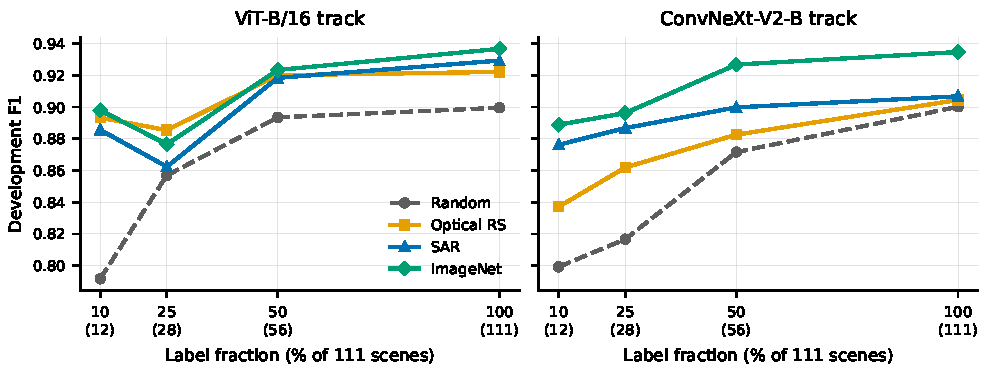
\includegraphics[width=\textwidth]{heldout_label_efficiency.pdf}
\caption{Development-F1 label-efficiency curves, one panel per track. Solid
lines are pretrained arms. The dashed gray line is the track's random floor.
Values are seed-0 point estimates. We draw no uncertainty ribbon.}
\label{fig:label-efficiency}
\end{figure}

\paragraph{Label-efficiency curves and transfer gains.}

At 12 scenes, every pretrained arm beats its random floor in both tracks.
The ViT gains are \HevDeltaFTenViTOptical{} for optical,
\HevDeltaFTenViTSar{} for SAR, and \HevDeltaFTenViTImageNet{} for ImageNet
(Eq.~\eqref{eq:gain} and Fig.~\ref{fig:transfer-gains}). The CNN gains are
\HevDeltaFTenCNNOptical{}, \HevDeltaFTenCNNSar{}, and
\HevDeltaFTenCNNImageNet. CNN-optical now beats random at every budget
because of the input adapter (Sect.~\ref{sec:methods}).

At 12 scenes, ViT-ImageNet comes within 0.002 of the full-data ViT random
floor (\HevDevFViTImageNetTen{} versus \HevDevFViTRandomHundred).

\paragraph{Source-domain contrasts and architecture generality.}

The SAR--optical ranking depends on the backbone
(Eq.~\eqref{eq:contrast} and Fig.~\ref{fig:transfer-gains}). On
development F1, CNN-SAR leads CNN-optical at every budget, but the gap
shrinks from \HevDevFCNNSarTen{} versus \HevDevFCNNOpticalTen{} at 12 scenes
to \HevDevFCNNSarHundred{} versus \HevDevFCNNOpticalHundred{} at 111. The
BigEarthNet Sentinel-1 and Sentinel-2 checkpoints share their architecture,
dataset family, and supervised task, which makes this the cleanest modality
comparison in the study. In the ViT track, optical leads SAR at 10\%, 25\%,
and 50\%, and SAR leads only at 100\%. The scarce-label SAR--optical order
therefore does not replicate across architectures. The ViT checkpoints also
differ in objective and source corpus, so their ranking cannot identify a
modality-only effect.

\paragraph{Held-out test results.}

\ifHevTestComplete
All 32 cells were scored once on the frozen 16-scene test split with their
development-bound thresholds and \HevTestInferencePrecision{} inference.
The test column appears only after every result validates against the frozen
cohort. Test F1 is lower than development F1 for every cell, by 0.029 to
0.142 and \HevTestMeanGap{} on average, as selection on eight scenes leads
one to expect.

Every pretrained arm still beats its random floor at 12 scenes. In the CNN
track, SAR leads optical at 12, 28, and 56 scenes (\HevTestFCNNSarTen{}
versus \HevTestFCNNOpticalTen{} at 12) and trails it at 111
(\HevTestFCNNSarHundred{} versus \HevTestFCNNOpticalHundred). In the ViT
track, the two arms tie at 12 scenes (\HevTestFViTSarTen{} versus
\HevTestFViTOpticalTen), optical leads at 28, and SAR leads at 56 and 111.
The full-data winner changes in one track: ViT-SAR reaches
\HevTestFViTSarHundred, above ImageNet's \HevTestFViTImageNetHundred, while
CNN-ImageNet keeps its lead at \HevTestFCNNImageNetHundred. On test, 28
pretrained scenes already match the full-data random floor in both tracks.
The 28 cells outside the CNN-optical arm repeat the recipe and seed of an
earlier cohort (code \texttt{1a82d508}), yet their test F1 differs from it
by up to 0.043, so we treat contrasts below about 0.04 as run-to-run
variation.

The predeclared monotonicity gate failed on two SAR test curves. ViT-SAR
falls from \HevTestFViTSarTen{} at 10\% to \HevTestFViTSarTwentyFive{} at
25\%, and CNN-SAR falls from \HevTestFCNNSarFifty{} at 50\% to
\HevTestFCNNSarHundred{} at 100\% although its development F1 rises. Both
declines exceed the allowed 0.02, so the experiment does not establish a
monotone label-efficiency curve. The final evaluation proceeded with this
failure disclosed, with no retraining and no threshold tuning.
\else
The 16-scene test split has not been scored in this build. The held-out
contract first freezes the 32-cell cohort. It then applies each cell's
development-bound threshold and writes one immutable result. The generator
admits test values only when all 32 results validate.
\fi

\paragraph{Once-only human-verified evaluation.}

\ifHevFinalEval
\begin{table}[t]
\centering
\caption{F1 on the \HevFinalScenes{} human-verified scenes, scored once
with each cell's development-bound threshold. Appendix~\ref{app:inventory}
adds recall, dark-vessel recall, and near-shore F1.}
\label{tab:final}
\small
\setlength{\tabcolsep}{5pt}
\begin{tabular}{@{}llcccc@{}}
\toprule
Track & Initialization & 10\% (12) & 25\% (28) & 50\% (56) & 100\% (111) \\
\midrule
ViT-B/16 & Random & \HevFinalFViTRandomTen & \HevFinalFViTRandomTwentyFive & \HevFinalFViTRandomFifty & \HevFinalFViTRandomHundred \\
 & Optical & \HevFinalFViTOpticalTen & \HevFinalFViTOpticalTwentyFive & \HevFinalFViTOpticalFifty & \HevFinalFViTOpticalHundred \\
 & SAR & \HevFinalFViTSarTen & \HevFinalFViTSarTwentyFive & \HevFinalFViTSarFifty & \HevFinalFViTSarHundred \\
 & ImageNet & \HevFinalFViTImageNetTen & \HevFinalFViTImageNetTwentyFive & \HevFinalFViTImageNetFifty & \HevFinalFViTImageNetHundred \\
\midrule
ConvNeXt-V2-B & Random & \HevFinalFCNNRandomTen & \HevFinalFCNNRandomTwentyFive & \HevFinalFCNNRandomFifty & \HevFinalFCNNRandomHundred \\
 & Optical & \HevFinalFCNNOpticalTen & \HevFinalFCNNOpticalTwentyFive & \HevFinalFCNNOpticalFifty & \HevFinalFCNNOpticalHundred \\
 & SAR & \HevFinalFCNNSarTen & \HevFinalFCNNSarTwentyFive & \HevFinalFCNNSarFifty & \HevFinalFCNNSarHundred \\
 & ImageNet & \HevFinalFCNNImageNetTen & \HevFinalFCNNImageNetTwentyFive & \HevFinalFCNNImageNetFifty & \HevFinalFCNNImageNetHundred \\
\bottomrule
\end{tabular}
\end{table}

All 32 cells were scored once on the \HevFinalScenes{} human-verified
scenes (Table~\ref{tab:final}). They hold \HevFinalPositives{} vessels, of
which \HevFinalDarkSupport{} are dark and \HevFinalNearShoreSupport{} lie
within 2\,km of shore. F1 falls to \HevFinalFMin--\HevFinalFMax, on average
\HevFinalMeanTestGap{} below test F1. Precision stays between
\HevFinalPrecisionMin{} and \HevFinalPrecisionMax, but recall drops to
\HevFinalRecallMin--\HevFinalRecallMax: the detectors miss vessels rather
than over-detect. No cell exceeds
\HevFinalNearShoreFMax{} near-shore F1 or \HevFinalDarkRecallMax{}
dark-vessel recall. The training labels explain much of this gap: only
\HevTrainNearShorePositives{} of the \HevTrainPositives{} training vessels
(\HevTrainNearShorePct\%) lie within 2\,km of shore, against
\HevFinalNearShorePct\% of the verified vessels.

The 12-scene pretraining advantage survives this shift: the six gains over
random range from \HevDeltaFinalTenCNNOptical{} to
\HevDeltaFinalTenViTImageNet, and ViT-ImageNet at 12 scenes matches the ViT
random floor at 111 (\HevFinalFViTImageNetTen{} versus
\HevFinalFViTRandomHundred). CNN-SAR again leads optical only with few
labels (\HevFinalFCNNSarTen{} versus \HevFinalFCNNOpticalTen{} at 12 scenes,
\HevFinalFCNNSarHundred{} versus \HevFinalFCNNOpticalHundred{} at 111). Both
SAR declines from the test split recur on this set and grow larger.
\else
The 50 human-verified scenes remain sealed. Dark-vessel recall and near-shore
performance are defined only on that set, so neither result is available in
this report.
\fi

\section{Conclusion and Future Work}

Pretraining improved label efficiency where labels are scarcest. At 12
scenes, all six pretrained checkpoints beat their random floors on
development selection\ifHevTestComplete, on the held-out test split\fi\ifHevFinalEval,
and on the once-only human-verified set\fi. No single source won across both
backbones and all evaluation stages. In the CNN track, SAR pretraining leads
optical pretraining with few labels, and the lead shrinks as labels
grow.\ifHevTestComplete{} On test it reverses at 111 scenes.\fi{} The ViT
track shows no stable SAR--optical order. The input adapter mattered as much as the source domain: a seeded
three-channel stem turned the ten-band BigEarthNet-S2 checkpoint from no
gain into a gain at every budget, so cross-sensor studies should report the
adapter rule.

\ifHevTestComplete
The failed monotonicity gate and rerun variation of up to 0.043 test F1
limit these conclusions. The grid is a set of descriptive seed-0 point
estimates, not evidence that performance improves monotonically with more
labels.
\else
The frozen 16-scene test split remains the next held-out stage. It will use
each cell's development-bound threshold without retuning.
\fi

\ifHevFinalEval
The human-verified set exposes the main open problem. Every detector loses
about \HevFinalMeanTestGap{} F1 against test, and no cell exceeds
\HevFinalDarkRecallMax{} dark-vessel recall or \HevFinalNearShoreFMax{}
near-shore F1. Only \HevTrainNearShorePct\% of training vessels lie near
shore, against \HevFinalNearShorePct\% of verified ones, so the gap reflects
the training labels as much as coastal clutter.
\else
The 50 human-verified scenes remain sealed, so dark-vessel recall and
near-shore performance are not yet measured.
\fi

Each cell uses one seed and eight selection scenes, and the ViT checkpoints
differ in objective and corpus, so the results compare released checkpoints
rather than a causal domain effect. Future work should add seeds,
near-shore labels, an independent test region, and matched objectives.

\label{mainbody:end}
\clearpage
\bibliographystyle{abbrv}
\bibliography{references}
\clearpage
\appendix
\section{Full Evidence Inventory}
\label{app:inventory}

Table~\ref{tab:inventory} lists every cell: development-selection F1, the
checkpoint-bound operating threshold, the epoch of the selected checkpoint,
the epochs run, measured GPU-hours, and held-out test F1 where admitted.
\ifHevFinalEval Table~\ref{tab:final-inventory} lists the once-only
human-verified results.\fi
The build re-derives all values from the committed cohort, markers,
training curves, and runtime receipts. Dashes mean the fail-closed
generator admitted no value, never zero performance.

\begin{table}[h]
\centering
\caption{Per-cell evidence inventory for development selection. The test
column is admitted only when all 32 immutable held-out results validate.}
\label{tab:inventory}
\scriptsize
\setlength{\tabcolsep}{4pt}
\renewcommand{\arraystretch}{0.95}
\begin{tabular}{@{}llcccccc@{}}
\toprule
Cell & Budget & Dev F1 & Threshold & Best ep. & Epochs & GPU-h & Test F1 \\
\midrule
ViT random & 10\% & \HevDevFViTRandomTen & \HevThrViTRandomTen & \HevEpochViTRandomTen & \HevEpochsRunViTRandomTen & \HevHoursViTRandomTen & \HevTestFViTRandomTen \\
ViT random & 25\% & \HevDevFViTRandomTwentyFive & \HevThrViTRandomTwentyFive & \HevEpochViTRandomTwentyFive & \HevEpochsRunViTRandomTwentyFive & \HevHoursViTRandomTwentyFive & \HevTestFViTRandomTwentyFive \\
ViT random & 50\% & \HevDevFViTRandomFifty & \HevThrViTRandomFifty & \HevEpochViTRandomFifty & \HevEpochsRunViTRandomFifty & \HevHoursViTRandomFifty & \HevTestFViTRandomFifty \\
ViT random & 100\% & \HevDevFViTRandomHundred & \HevThrViTRandomHundred & \HevEpochViTRandomHundred & \HevEpochsRunViTRandomHundred & \HevHoursViTRandomHundred & \HevTestFViTRandomHundred \\
ViT optical & 10\% & \HevDevFViTOpticalTen & \HevThrViTOpticalTen & \HevEpochViTOpticalTen & \HevEpochsRunViTOpticalTen & \HevHoursViTOpticalTen & \HevTestFViTOpticalTen \\
ViT optical & 25\% & \HevDevFViTOpticalTwentyFive & \HevThrViTOpticalTwentyFive & \HevEpochViTOpticalTwentyFive & \HevEpochsRunViTOpticalTwentyFive & \HevHoursViTOpticalTwentyFive & \HevTestFViTOpticalTwentyFive \\
ViT optical & 50\% & \HevDevFViTOpticalFifty & \HevThrViTOpticalFifty & \HevEpochViTOpticalFifty & \HevEpochsRunViTOpticalFifty & \HevHoursViTOpticalFifty & \HevTestFViTOpticalFifty \\
ViT optical & 100\% & \HevDevFViTOpticalHundred & \HevThrViTOpticalHundred & \HevEpochViTOpticalHundred & \HevEpochsRunViTOpticalHundred & \HevHoursViTOpticalHundred & \HevTestFViTOpticalHundred \\
ViT SAR & 10\% & \HevDevFViTSarTen & \HevThrViTSarTen & \HevEpochViTSarTen & \HevEpochsRunViTSarTen & \HevHoursViTSarTen & \HevTestFViTSarTen \\
ViT SAR & 25\% & \HevDevFViTSarTwentyFive & \HevThrViTSarTwentyFive & \HevEpochViTSarTwentyFive & \HevEpochsRunViTSarTwentyFive & \HevHoursViTSarTwentyFive & \HevTestFViTSarTwentyFive \\
ViT SAR & 50\% & \HevDevFViTSarFifty & \HevThrViTSarFifty & \HevEpochViTSarFifty & \HevEpochsRunViTSarFifty & \HevHoursViTSarFifty & \HevTestFViTSarFifty \\
ViT SAR & 100\% & \HevDevFViTSarHundred & \HevThrViTSarHundred & \HevEpochViTSarHundred & \HevEpochsRunViTSarHundred & \HevHoursViTSarHundred & \HevTestFViTSarHundred \\
ViT ImageNet & 10\% & \HevDevFViTImageNetTen & \HevThrViTImageNetTen & \HevEpochViTImageNetTen & \HevEpochsRunViTImageNetTen & \HevHoursViTImageNetTen & \HevTestFViTImageNetTen \\
ViT ImageNet & 25\% & \HevDevFViTImageNetTwentyFive & \HevThrViTImageNetTwentyFive & \HevEpochViTImageNetTwentyFive & \HevEpochsRunViTImageNetTwentyFive & \HevHoursViTImageNetTwentyFive & \HevTestFViTImageNetTwentyFive \\
ViT ImageNet & 50\% & \HevDevFViTImageNetFifty & \HevThrViTImageNetFifty & \HevEpochViTImageNetFifty & \HevEpochsRunViTImageNetFifty & \HevHoursViTImageNetFifty & \HevTestFViTImageNetFifty \\
ViT ImageNet & 100\% & \HevDevFViTImageNetHundred & \HevThrViTImageNetHundred & \HevEpochViTImageNetHundred & \HevEpochsRunViTImageNetHundred & \HevHoursViTImageNetHundred & \HevTestFViTImageNetHundred \\
\midrule
CNN random & 10\% & \HevDevFCNNRandomTen & \HevThrCNNRandomTen & \HevEpochCNNRandomTen & \HevEpochsRunCNNRandomTen & \HevHoursCNNRandomTen & \HevTestFCNNRandomTen \\
CNN random & 25\% & \HevDevFCNNRandomTwentyFive & \HevThrCNNRandomTwentyFive & \HevEpochCNNRandomTwentyFive & \HevEpochsRunCNNRandomTwentyFive & \HevHoursCNNRandomTwentyFive & \HevTestFCNNRandomTwentyFive \\
CNN random & 50\% & \HevDevFCNNRandomFifty & \HevThrCNNRandomFifty & \HevEpochCNNRandomFifty & \HevEpochsRunCNNRandomFifty & \HevHoursCNNRandomFifty & \HevTestFCNNRandomFifty \\
CNN random & 100\% & \HevDevFCNNRandomHundred & \HevThrCNNRandomHundred & \HevEpochCNNRandomHundred & \HevEpochsRunCNNRandomHundred & \HevHoursCNNRandomHundred & \HevTestFCNNRandomHundred \\
CNN optical & 10\% & \HevDevFCNNOpticalTen & \HevThrCNNOpticalTen & \HevEpochCNNOpticalTen & \HevEpochsRunCNNOpticalTen & \HevHoursCNNOpticalTen & \HevTestFCNNOpticalTen \\
CNN optical & 25\% & \HevDevFCNNOpticalTwentyFive & \HevThrCNNOpticalTwentyFive & \HevEpochCNNOpticalTwentyFive & \HevEpochsRunCNNOpticalTwentyFive & \HevHoursCNNOpticalTwentyFive & \HevTestFCNNOpticalTwentyFive \\
CNN optical & 50\% & \HevDevFCNNOpticalFifty & \HevThrCNNOpticalFifty & \HevEpochCNNOpticalFifty & \HevEpochsRunCNNOpticalFifty & \HevHoursCNNOpticalFifty & \HevTestFCNNOpticalFifty \\
CNN optical & 100\% & \HevDevFCNNOpticalHundred & \HevThrCNNOpticalHundred & \HevEpochCNNOpticalHundred & \HevEpochsRunCNNOpticalHundred & \HevHoursCNNOpticalHundred & \HevTestFCNNOpticalHundred \\
CNN SAR & 10\% & \HevDevFCNNSarTen & \HevThrCNNSarTen & \HevEpochCNNSarTen & \HevEpochsRunCNNSarTen & \HevHoursCNNSarTen & \HevTestFCNNSarTen \\
CNN SAR & 25\% & \HevDevFCNNSarTwentyFive & \HevThrCNNSarTwentyFive & \HevEpochCNNSarTwentyFive & \HevEpochsRunCNNSarTwentyFive & \HevHoursCNNSarTwentyFive & \HevTestFCNNSarTwentyFive \\
CNN SAR & 50\% & \HevDevFCNNSarFifty & \HevThrCNNSarFifty & \HevEpochCNNSarFifty & \HevEpochsRunCNNSarFifty & \HevHoursCNNSarFifty & \HevTestFCNNSarFifty \\
CNN SAR & 100\% & \HevDevFCNNSarHundred & \HevThrCNNSarHundred & \HevEpochCNNSarHundred & \HevEpochsRunCNNSarHundred & \HevHoursCNNSarHundred & \HevTestFCNNSarHundred \\
CNN ImageNet & 10\% & \HevDevFCNNImageNetTen & \HevThrCNNImageNetTen & \HevEpochCNNImageNetTen & \HevEpochsRunCNNImageNetTen & \HevHoursCNNImageNetTen & \HevTestFCNNImageNetTen \\
CNN ImageNet & 25\% & \HevDevFCNNImageNetTwentyFive & \HevThrCNNImageNetTwentyFive & \HevEpochCNNImageNetTwentyFive & \HevEpochsRunCNNImageNetTwentyFive & \HevHoursCNNImageNetTwentyFive & \HevTestFCNNImageNetTwentyFive \\
CNN ImageNet & 50\% & \HevDevFCNNImageNetFifty & \HevThrCNNImageNetFifty & \HevEpochCNNImageNetFifty & \HevEpochsRunCNNImageNetFifty & \HevHoursCNNImageNetFifty & \HevTestFCNNImageNetFifty \\
CNN ImageNet & 100\% & \HevDevFCNNImageNetHundred & \HevThrCNNImageNetHundred & \HevEpochCNNImageNetHundred & \HevEpochsRunCNNImageNetHundred & \HevHoursCNNImageNetHundred & \HevTestFCNNImageNetHundred \\
\bottomrule
\end{tabular}
\end{table}

\ifHevFinalEval
\begin{table}[h]
\centering
\caption{Per-cell results on the 50 human-verified scenes, scored once with
each cell's development-bound threshold. Dark-vessel recall covers the
\HevFinalDarkSupport{} vessels without an AIS match; near-shore F1 covers
the \HevFinalNearShoreSupport{} vessels within 2\,km of shore.}
\label{tab:final-inventory}
\scriptsize
\setlength{\tabcolsep}{4pt}
\renewcommand{\arraystretch}{0.95}
\begin{tabular}{@{}llcccc@{}}
\toprule
Cell & Budget & Final F1 & Recall & Dark recall & Near-shore F1 \\
\midrule
ViT random & 10\% & \HevFinalFViTRandomTen & \HevFinalRecallViTRandomTen & \HevFinalDarkRecallViTRandomTen & \HevFinalNearShoreFViTRandomTen \\
ViT random & 25\% & \HevFinalFViTRandomTwentyFive & \HevFinalRecallViTRandomTwentyFive & \HevFinalDarkRecallViTRandomTwentyFive & \HevFinalNearShoreFViTRandomTwentyFive \\
ViT random & 50\% & \HevFinalFViTRandomFifty & \HevFinalRecallViTRandomFifty & \HevFinalDarkRecallViTRandomFifty & \HevFinalNearShoreFViTRandomFifty \\
ViT random & 100\% & \HevFinalFViTRandomHundred & \HevFinalRecallViTRandomHundred & \HevFinalDarkRecallViTRandomHundred & \HevFinalNearShoreFViTRandomHundred \\
ViT optical & 10\% & \HevFinalFViTOpticalTen & \HevFinalRecallViTOpticalTen & \HevFinalDarkRecallViTOpticalTen & \HevFinalNearShoreFViTOpticalTen \\
ViT optical & 25\% & \HevFinalFViTOpticalTwentyFive & \HevFinalRecallViTOpticalTwentyFive & \HevFinalDarkRecallViTOpticalTwentyFive & \HevFinalNearShoreFViTOpticalTwentyFive \\
ViT optical & 50\% & \HevFinalFViTOpticalFifty & \HevFinalRecallViTOpticalFifty & \HevFinalDarkRecallViTOpticalFifty & \HevFinalNearShoreFViTOpticalFifty \\
ViT optical & 100\% & \HevFinalFViTOpticalHundred & \HevFinalRecallViTOpticalHundred & \HevFinalDarkRecallViTOpticalHundred & \HevFinalNearShoreFViTOpticalHundred \\
ViT SAR & 10\% & \HevFinalFViTSarTen & \HevFinalRecallViTSarTen & \HevFinalDarkRecallViTSarTen & \HevFinalNearShoreFViTSarTen \\
ViT SAR & 25\% & \HevFinalFViTSarTwentyFive & \HevFinalRecallViTSarTwentyFive & \HevFinalDarkRecallViTSarTwentyFive & \HevFinalNearShoreFViTSarTwentyFive \\
ViT SAR & 50\% & \HevFinalFViTSarFifty & \HevFinalRecallViTSarFifty & \HevFinalDarkRecallViTSarFifty & \HevFinalNearShoreFViTSarFifty \\
ViT SAR & 100\% & \HevFinalFViTSarHundred & \HevFinalRecallViTSarHundred & \HevFinalDarkRecallViTSarHundred & \HevFinalNearShoreFViTSarHundred \\
ViT ImageNet & 10\% & \HevFinalFViTImageNetTen & \HevFinalRecallViTImageNetTen & \HevFinalDarkRecallViTImageNetTen & \HevFinalNearShoreFViTImageNetTen \\
ViT ImageNet & 25\% & \HevFinalFViTImageNetTwentyFive & \HevFinalRecallViTImageNetTwentyFive & \HevFinalDarkRecallViTImageNetTwentyFive & \HevFinalNearShoreFViTImageNetTwentyFive \\
ViT ImageNet & 50\% & \HevFinalFViTImageNetFifty & \HevFinalRecallViTImageNetFifty & \HevFinalDarkRecallViTImageNetFifty & \HevFinalNearShoreFViTImageNetFifty \\
ViT ImageNet & 100\% & \HevFinalFViTImageNetHundred & \HevFinalRecallViTImageNetHundred & \HevFinalDarkRecallViTImageNetHundred & \HevFinalNearShoreFViTImageNetHundred \\
\midrule
CNN random & 10\% & \HevFinalFCNNRandomTen & \HevFinalRecallCNNRandomTen & \HevFinalDarkRecallCNNRandomTen & \HevFinalNearShoreFCNNRandomTen \\
CNN random & 25\% & \HevFinalFCNNRandomTwentyFive & \HevFinalRecallCNNRandomTwentyFive & \HevFinalDarkRecallCNNRandomTwentyFive & \HevFinalNearShoreFCNNRandomTwentyFive \\
CNN random & 50\% & \HevFinalFCNNRandomFifty & \HevFinalRecallCNNRandomFifty & \HevFinalDarkRecallCNNRandomFifty & \HevFinalNearShoreFCNNRandomFifty \\
CNN random & 100\% & \HevFinalFCNNRandomHundred & \HevFinalRecallCNNRandomHundred & \HevFinalDarkRecallCNNRandomHundred & \HevFinalNearShoreFCNNRandomHundred \\
CNN optical & 10\% & \HevFinalFCNNOpticalTen & \HevFinalRecallCNNOpticalTen & \HevFinalDarkRecallCNNOpticalTen & \HevFinalNearShoreFCNNOpticalTen \\
CNN optical & 25\% & \HevFinalFCNNOpticalTwentyFive & \HevFinalRecallCNNOpticalTwentyFive & \HevFinalDarkRecallCNNOpticalTwentyFive & \HevFinalNearShoreFCNNOpticalTwentyFive \\
CNN optical & 50\% & \HevFinalFCNNOpticalFifty & \HevFinalRecallCNNOpticalFifty & \HevFinalDarkRecallCNNOpticalFifty & \HevFinalNearShoreFCNNOpticalFifty \\
CNN optical & 100\% & \HevFinalFCNNOpticalHundred & \HevFinalRecallCNNOpticalHundred & \HevFinalDarkRecallCNNOpticalHundred & \HevFinalNearShoreFCNNOpticalHundred \\
CNN SAR & 10\% & \HevFinalFCNNSarTen & \HevFinalRecallCNNSarTen & \HevFinalDarkRecallCNNSarTen & \HevFinalNearShoreFCNNSarTen \\
CNN SAR & 25\% & \HevFinalFCNNSarTwentyFive & \HevFinalRecallCNNSarTwentyFive & \HevFinalDarkRecallCNNSarTwentyFive & \HevFinalNearShoreFCNNSarTwentyFive \\
CNN SAR & 50\% & \HevFinalFCNNSarFifty & \HevFinalRecallCNNSarFifty & \HevFinalDarkRecallCNNSarFifty & \HevFinalNearShoreFCNNSarFifty \\
CNN SAR & 100\% & \HevFinalFCNNSarHundred & \HevFinalRecallCNNSarHundred & \HevFinalDarkRecallCNNSarHundred & \HevFinalNearShoreFCNNSarHundred \\
CNN ImageNet & 10\% & \HevFinalFCNNImageNetTen & \HevFinalRecallCNNImageNetTen & \HevFinalDarkRecallCNNImageNetTen & \HevFinalNearShoreFCNNImageNetTen \\
CNN ImageNet & 25\% & \HevFinalFCNNImageNetTwentyFive & \HevFinalRecallCNNImageNetTwentyFive & \HevFinalDarkRecallCNNImageNetTwentyFive & \HevFinalNearShoreFCNNImageNetTwentyFive \\
CNN ImageNet & 50\% & \HevFinalFCNNImageNetFifty & \HevFinalRecallCNNImageNetFifty & \HevFinalDarkRecallCNNImageNetFifty & \HevFinalNearShoreFCNNImageNetFifty \\
CNN ImageNet & 100\% & \HevFinalFCNNImageNetHundred & \HevFinalRecallCNNImageNetHundred & \HevFinalDarkRecallCNNImageNetHundred & \HevFinalNearShoreFCNNImageNetHundred \\
\bottomrule
\end{tabular}
\end{table}
\fi

The sanitized operator status snapshot from the earlier cohort's deadline
remains committed beside the evidence tree as a historical record of
execution state. It does not describe the cohort reported here.

\clearpage
\section{Study Data and Figures}
\label{app:figures}

\begin{figure}[H]
\centering
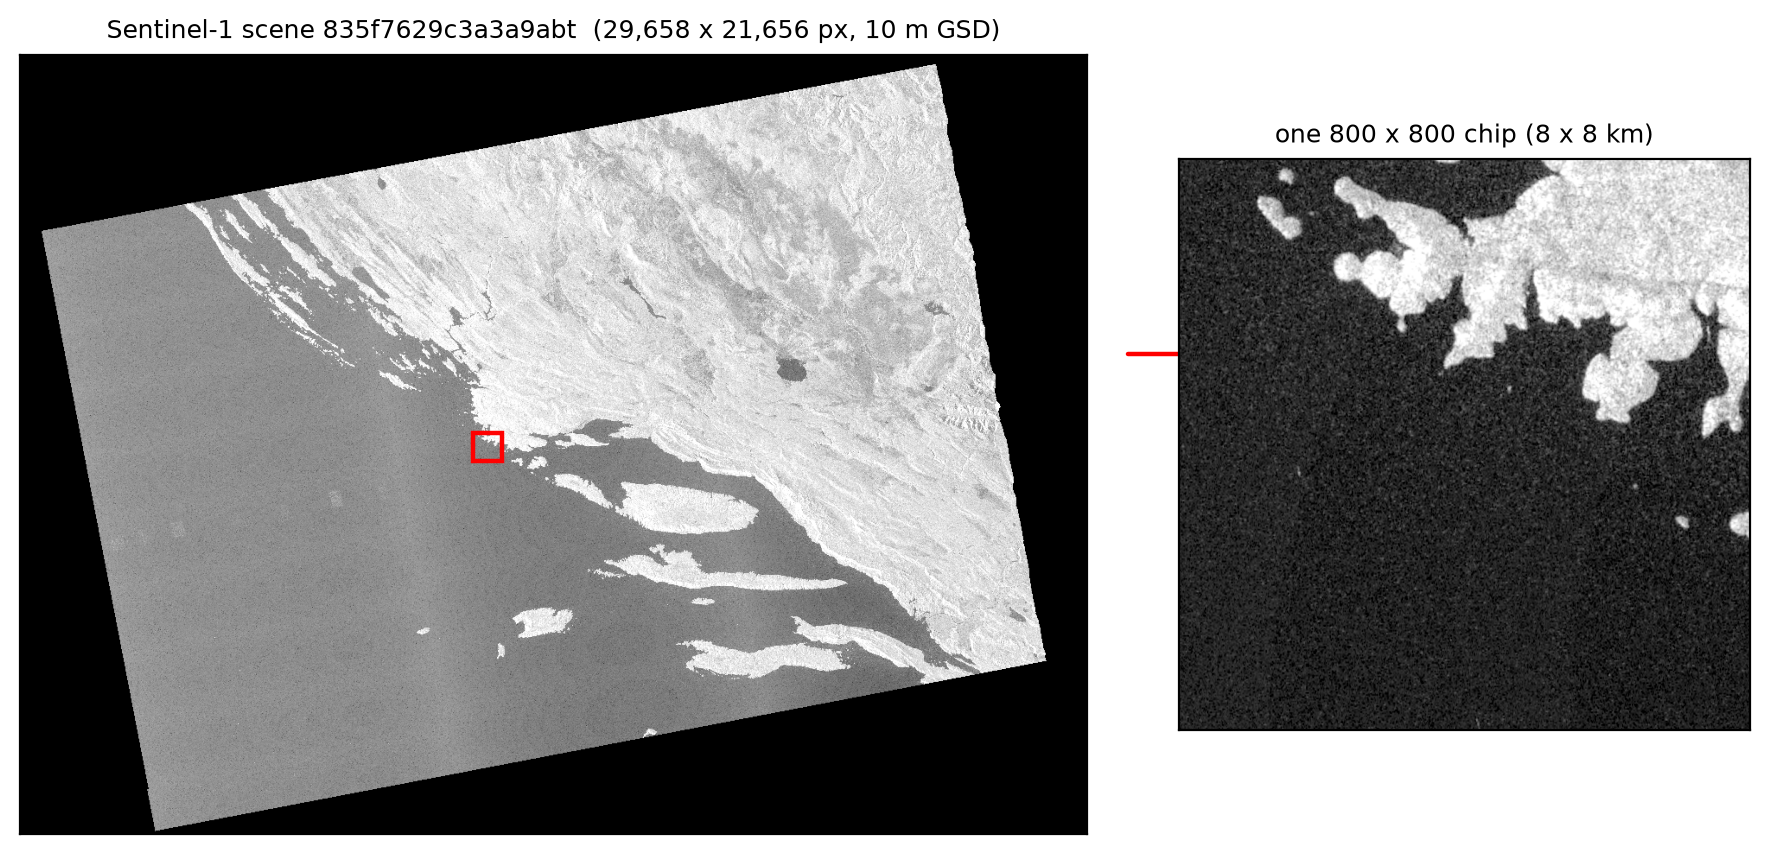
\includegraphics[width=0.9\textwidth]{static/scene_context.png}\\[4pt]
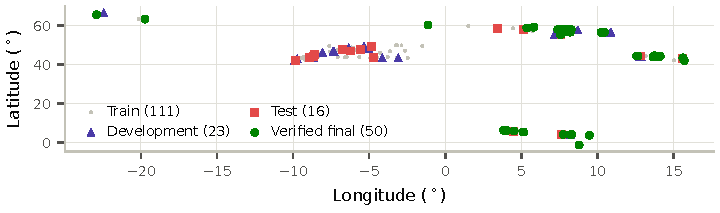
\includegraphics[width=0.9\textwidth]{static/scene_map.pdf}
\caption{Study data. Top: scale context for one study scene, a full
Sentinel-1 ground-range-detected scene and the single $800\times800$ chip
($8\times8$\,km) marked by the red box. Vessels occupy only a few pixels at
this scale. Bottom: scene centroids of the frozen splits, computed from the
label records. Sentinel-1 revisits place held-out scenes near training
scenes, which is why Sect.~\ref{sec:data} reports in-region
generalization.}
\label{fig:study-data}
\end{figure}

\begin{figure}[H]
\centering
\setlength{\fboxsep}{3pt}
\fbox{\parbox[c][1.75cm][c]{0.26\textwidth}{\centering\scriptsize
\textbf{Frozen scenes}\\[2pt]
111 train / 23 dev / 16 test\\
Nested 12, 28, 56, 111\\
50 verified, reserved once}}
\hfill$\Longrightarrow$\hfill
\fbox{\parbox[c][1.75cm][c]{0.28\textwidth}{\centering\scriptsize
\textbf{Two matched tracks}\\[2pt]
ViT-B/16: random, optical, SAR, ImageNet\\
ConvNeXt-V2-B: same roles}}
\hfill$\Longrightarrow$\hfill
\fbox{\parbox[c][1.75cm][c]{0.25\textwidth}{\centering\scriptsize
\textbf{One detector contract}\\[2pt]
Shared input, head, optimizer, seed, FP32, and point scorer}}
\caption{Controlled study design. Initialization is the only variable within
each architecture track. Matched roles are compared descriptively across
tracks; the human-verified set stayed sealed until the cohort and the test
results were frozen, and was then scored once.}
\label{fig:study-design}
\end{figure}

\begin{figure}[H]
\centering
\resizebox{\textwidth}{!}{%
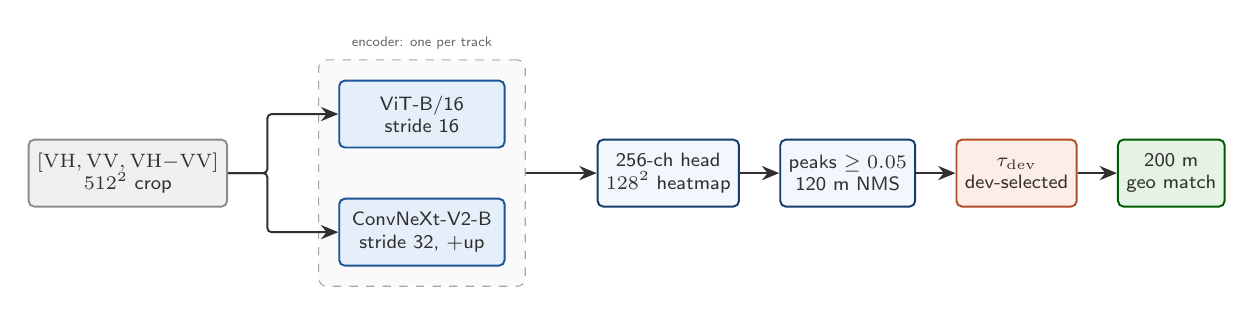
\begin{tikzpicture}[font=\sffamily\scriptsize, line width=0.7pt,
  >={Stealth[length=2.2mm, width=1.8mm]},
  stage/.style={draw, rounded corners=2pt, align=center, inner sep=3pt,
                minimum height=8.5mm, text=figink},
  data/.style={stage, fill=black!6, draw=black!45},
  enc/.style={stage, fill=figblue!12, draw=figblue!70!black, minimum width=21mm},
  neck/.style={stage, fill=figblue!6, draw=figblue!50!black},
  cal/.style={stage, fill=figorange!12, draw=figorange!75!black},
  endst/.style={stage, fill=figgreen!10, draw=figgreen!70!black},
  flow/.style={->, draw=figink, rounded corners=1.5pt}]
\node[data] (inp) {$[\mathrm{VH},\mathrm{VV},\mathrm{VH{-}VV}]$\\ $512^2$ crop};
\node[enc] (vit) at ($(inp.east)+(14mm,7.5mm)$) [anchor=west]
  {ViT-B/16\\ stride 16};
\node[enc] (cnn) at ($(inp.east)+(14mm,-7.5mm)$) [anchor=west]
  {ConvNeXt-V2-B\\ stride 32, $+$up};
\begin{scope}[on background layer]
\node[draw=black!35, dashed, rounded corners=3pt, inner sep=2.5mm,
      fit=(vit)(cnn), fill=black!2] (encbox) {};
\end{scope}
\node[anchor=south, font=\sffamily\tiny, text=black!60]
  at (encbox.north) {encoder: one per track};
\node[neck] (head) at ($(encbox.east)+(9mm,0)$) [anchor=west]
  {256-ch head\\ $128^2$ heatmap};
\node[neck, right=5mm of head] (dec) {peaks $\geq 0.05$\\ 120 m NMS};
\node[cal, right=5mm of dec] (op) {$\tau_{\mathrm{dev}}$\\ dev-selected};
\node[endst, right=5mm of op] (mat) {200 m\\ geo match};
\draw[flow] (inp.east) -- ($(inp.east)+(5mm,0)$) |- (vit.west);
\draw[flow] (inp.east) -- ($(inp.east)+(5mm,0)$) |- (cnn.west);
\draw[flow] (encbox.east) -- (head.west)
  node[midway, above, font=\sffamily\tiny, text=black!60] {};
\draw[flow] (head) -- (dec);
\draw[flow] (dec) -- (op);
\draw[flow] (op) -- (mat);
\end{tikzpicture}}
\caption{The shared detection path: only the encoder differs by track; one
head, decode rule, dev-selected threshold, and frozen scorer serve every arm.}
\label{fig:detector}
\end{figure}

\begin{figure}[H]
\centering
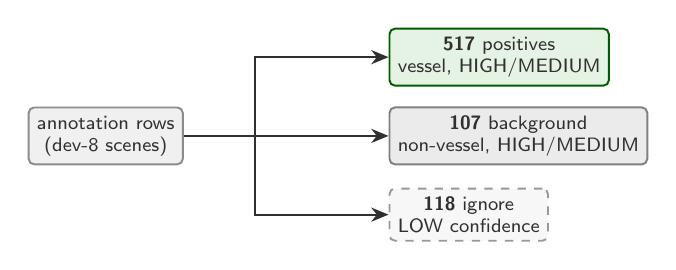
\begin{tikzpicture}[font=\sffamily\scriptsize, line width=0.7pt,
  >={Stealth[length=2.2mm, width=1.8mm]},
  stage/.style={draw, rounded corners=2pt, align=center, inner sep=3pt,
                text=figink},
  src/.style={stage, fill=black!6, draw=black!45},
  posbox/.style={stage, fill=figgreen!10, draw=figgreen!70!black},
  bg/.style={stage, fill=black!8, draw=black!50},
  ign/.style={stage, fill=black!3, draw=black!40, dashed},
  flow/.style={->, draw=figink}]
\node[src] (rows) {annotation rows\\ (dev-8 scenes)};
\node[posbox] (p) at ($(rows.east)+(26mm,10mm)$) [anchor=west]
  {\textbf{517} positives\\ vessel, HIGH/MEDIUM};
\node[bg] (n) at ($(rows.east)+(26mm,0)$) [anchor=west]
  {\textbf{107} background\\ non-vessel, HIGH/MEDIUM};
\node[ign] (i) at ($(rows.east)+(26mm,-10mm)$) [anchor=west]
  {\textbf{118} ignore\\ LOW confidence};
\draw[flow] (rows.east) -- ($(rows.east)+(9mm,0)$) |- (p.west);
\draw[flow] (rows.east) -- (n.west);
\draw[flow] (rows.east) -- ($(rows.east)+(9mm,0)$) |- (i.west);
\end{tikzpicture}
\caption{The corrected ground-truth contract on the training-time development
subset. A row is a positive only when \texttt{is\_vessel} is true at HIGH or
MEDIUM confidence; HIGH/MEDIUM non-vessels are background, and LOW-confidence
rows become ignore regions. Every H100 cell trained and evaluated under this
contract.}
\label{fig:gt-contract}
\end{figure}


\begin{figure}[H]
\centering
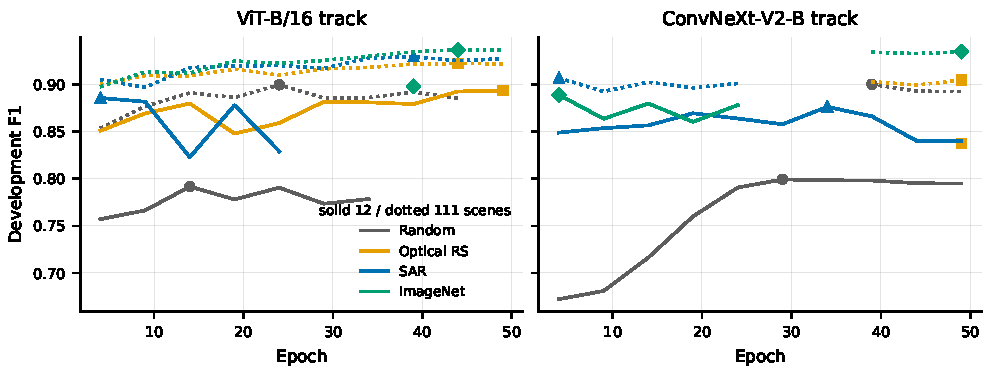
\includegraphics[width=\textwidth]{heldout_training_dynamics.pdf}
\caption{Development-F1 evaluation history for the smallest (12 scenes,
solid) and largest (111 scenes, dotted) budgets. A marker identifies each
selected checkpoint. The 12-scene ViT-ImageNet and CNN-optical curves were
not saved, so only their markers appear. Curves that start late belong to
resumed runs, which kept only post-resume evaluations. The SAR and ImageNet
CNN arms separate from the random floor in the first evaluations, and
checkpoint binding retains peaks that occur before the last evaluation.}
\label{fig:training-dynamics}
\end{figure}

\begin{figure}[H]
\centering
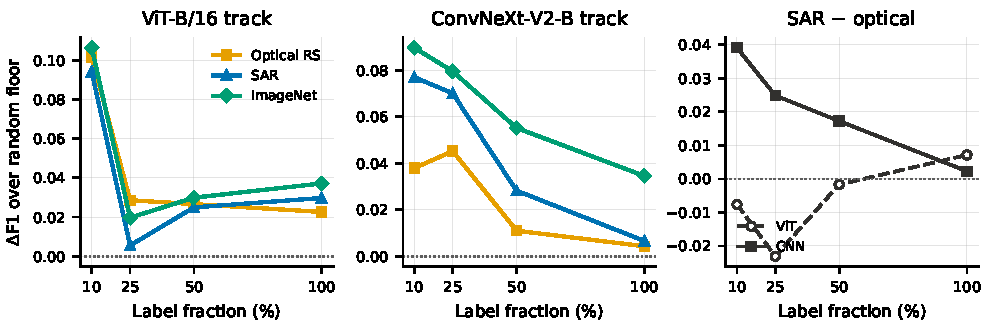
\includegraphics[width=\textwidth]{heldout_transfer_gains.pdf}
\caption{Left and center: transfer gain over the track-matched random floor
(Eq.~\eqref{eq:gain}) at each budget. Every gain is positive. Right: the
SAR--optical contrast (Eq.~\eqref{eq:contrast}). It is positive for the CNN
at every budget and shrinks toward zero at full data, but negative for the
ViT below full data, so the modality effect depends on the architecture.}
\label{fig:transfer-gains}
\end{figure}

\begin{figure}[H]
\centering
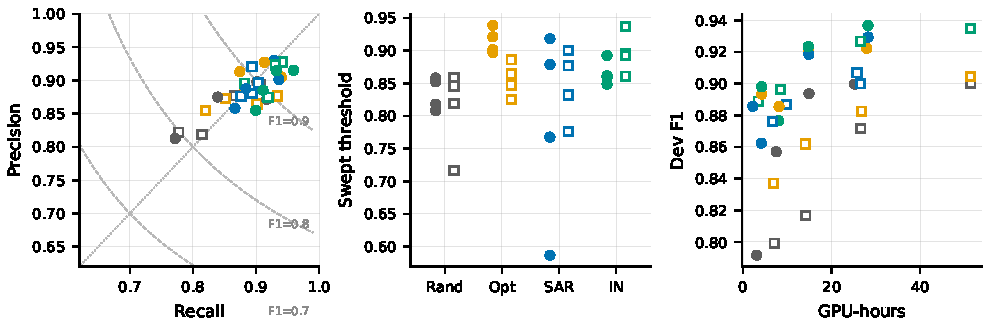
\includegraphics[width=\textwidth]{heldout_operating_points.pdf}
\caption{Operating points for all 32 cells. Filled circles show ViT, open
squares show CNN, and colors identify roles as in
Fig.~\ref{fig:label-efficiency}. The left panel shows precision--recall
positions with iso-F1 contours. The center panel shows the swept threshold
for each role. The right panel shows development F1 against measured
GPU-hours per cell.}
\label{fig:operating-points}
\end{figure}

\clearpage
\section{Extended Analysis}
\label{app:analysis}

\paragraph{Operating thresholds and calibration.}
Each cell selects its operating point on the training-time development
subset, and the cohort binds that point to the selected checkpoint.
Figure~\ref{fig:operating-points} shows all 32 of them. The recorded
thresholds vary widely (center panel): from \HevThrMinViT{} to
\HevThrMaxViT{} across the ViT cells and from \HevThrMinCNN{} to
\HevThrMaxCNN{} across the CNN cells. A single shared threshold would
therefore change the operating point for most arms. At the bound operating
point, precision exceeds recall in \HevCellsPrecOverRecall{} of the 32 cells
(left panel).

\paragraph{Training dynamics and cost.}
Figure~\ref{fig:training-dynamics} traces the development-F1 evaluation
history for the smallest and largest budgets. The SAR and ImageNet CNN arms
separate from the random floor in the first evaluations, and the ViT arms
begin closer together. The 12-scene CNN-optical curve was not saved, but its
selected checkpoint sits well above the random floor. Early
stopping, with a patience of four development evaluations, ended
\HevCellsEarlyStopped{} of the 32 cells before the 50-epoch cap. The median
best-checkpoint epoch is \HevMedianBestEpochViT{} for the ViT track and
\HevMedianBestEpochCNN{} for the CNN track. Fine-tuning cost also differs
between families. A ViT cell averaged \HevMeanCellHoursViT{} GPU-hours, and
a CNN cell averaged \HevMeanCellHoursCNN{} GPU-hours. The full matrix used
\HevGPUHours{} GPU-hours. Within each track, cost scales with the label
fraction, so the scarce-label comparisons also require the least
fine-tuning compute (Fig.~\ref{fig:operating-points}, right).

\paragraph{Why ViT-SAR dips at 28 scenes.}
The ViT-SAR (SARMAE) decline from 12 to 28 scenes appears on development,
test, and verified scores alike, so it belongs to the selected checkpoint,
not to one evaluation set. At both 12 and 28 scenes the run selected its
first development evaluation (epoch \HevEpochViTSarTen{} and epoch
\HevEpochViTSarTwentyFive), which falls as the five-epoch warm-up ends.
Training loss then kept falling while development F1 drifted down:
precision dropped and recall rose, the signature of overfitting a small
training set. With a patience of four evaluations, early stopping ended the
28-scene run after \HevEpochsRunViTSarTwentyFive{} epochs and kept the
warm-up checkpoint, whose threshold transferred poorly to held-out scenes.
SatDINO at 28 scenes dipped the same way but recovered just before patience
ran out and selected epoch \HevEpochViTOpticalTwentyFive. With 56 scenes,
SARMAE improved until epoch \HevEpochViTSarFifty{} and became the strongest
ViT cell on the verified set. The post-peak decline is about as large as
the bigger evaluation-to-evaluation swings of the eight-scene development
metric, so the stopping decision rests on a noisy signal. The retrained
cohort repeated the August values for this cell exactly, so the dip is
reproducible rather than nondeterministic.
Per-arm learning rates or longer patience may remove it; this study keeps
one shared recipe.

\paragraph{Qualitative example.}
\begin{figure}[H]
\centering
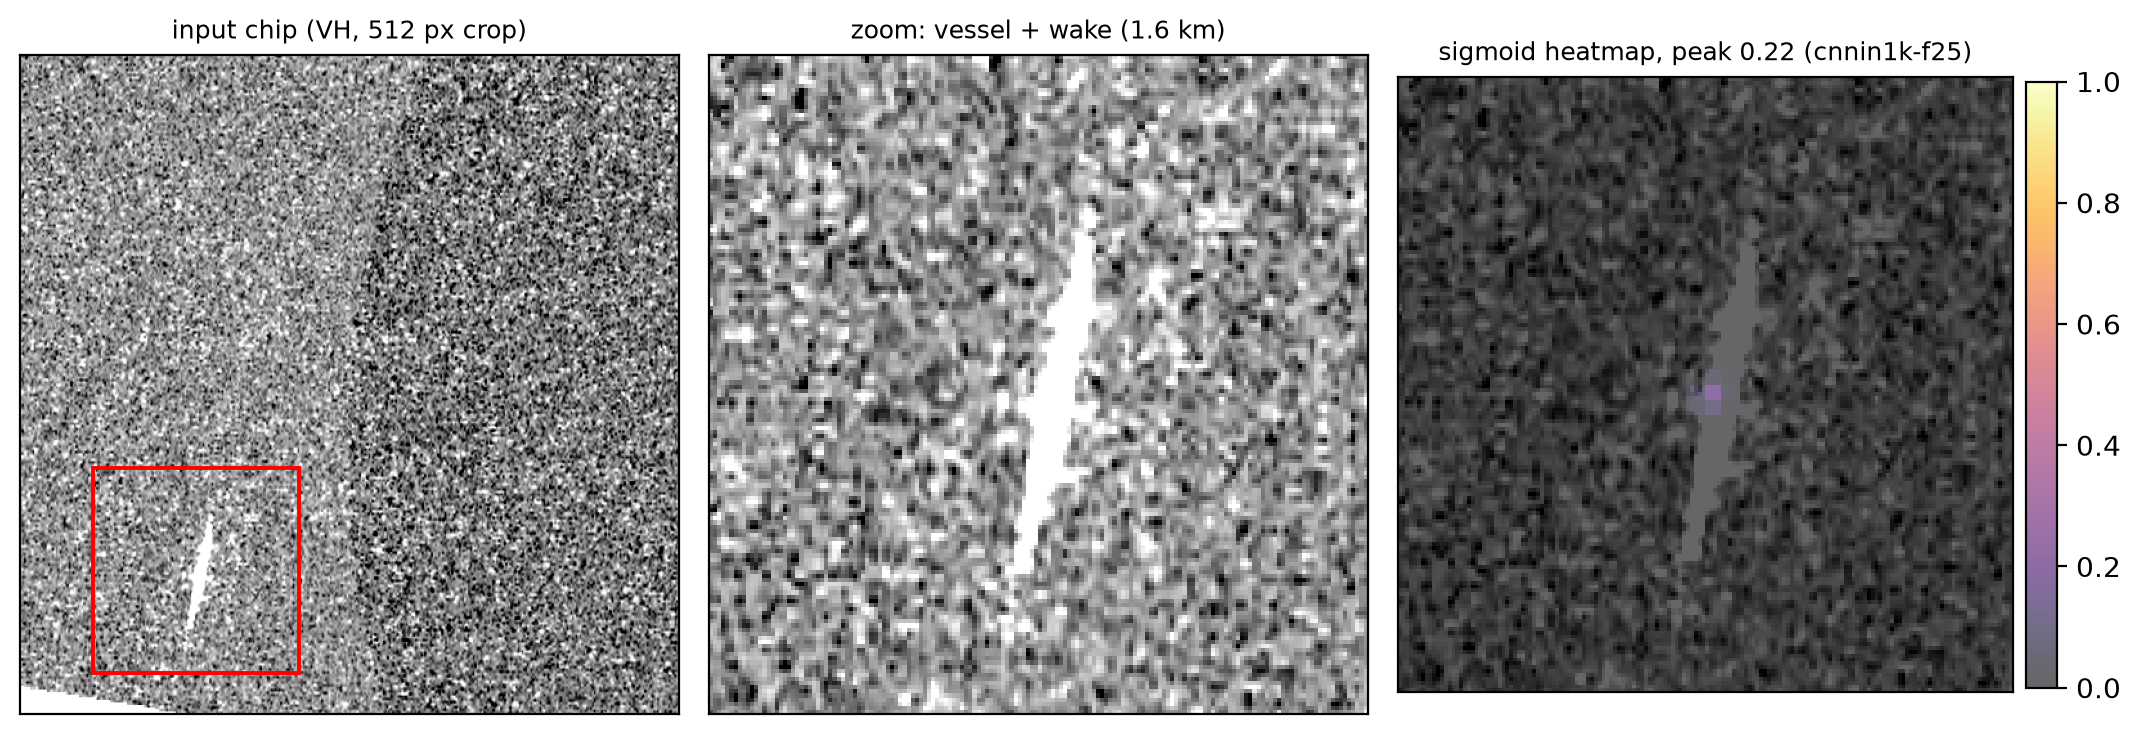
\includegraphics[width=0.92\textwidth]{static/heatmap_overlay.png}
\caption{A vessel-and-wake target and the shared detector's heatmap response
from a development-phase probe on this study's frozen splits (peak score
0.22). This sample is illustrative and not scored.}
\label{fig:qualitative}
\end{figure}
Figure~\ref{fig:qualitative} shows a detector response on a development
scene. The heatmap places a 0.22 peak on a clear vessel-and-wake target. This
example illustrates why candidate generation uses a 0.05 floor before the
per-cell threshold sweep. A fixed high candidate threshold would drop this
detection. The panel is illustrative and contributes no scored evidence to
the findings in Sect.~\ref{sec:results}.

\section{Reproducibility and Audit Record}
\label{app:audit}

The evidence tree records the frozen training cohort, each cell's
hash-bound completion marker, its full training curve, a sanitized runtime
receipt (H100 hardware class, source SHA, strict-FP32 backend state), and
the ground-truth audit receipt that binds every support count in
Table~\ref{tab:data-protocol} to the frozen split file. The generator
validates marker-to-cohort hashes, metric consistency, and curve agreement
before it writes a manuscript artifact. Two cells, 12-scene ViT-ImageNet
and 12-scene CNN-optical, ran their last development evaluation in a resume
that added no training step and did not save the curve. Their markers
hash-bind the recovery record, and the generator accepts the missing curve
only when that record selects exactly the marker's checkpoint and result.
Each human-verified result must hash to its entry in the final-evaluation
completion record and bind the cohort, the cell's test result, and its
threshold; the generator admits all 32 or none. Checkpoint bytes stay outside the
repository. We publish their SHA-256 bindings for archive verification.
The submission excludes imagery, labels, weights, checkpoints, run trees,
credentials, and private paths.

The detector uses 512-pixel crops, a stride-4 heatmap, Gaussian standard
deviation two output pixels, a candidate floor of 0.05, and 120\,m distance
NMS. Training uses at most 50 epochs with development evaluation every five
epochs. The project fixes seed 0 and reports point estimates without
uncertainty bands.

\end{document}
